%%%%%%%%%%%%%%%%%%%%%%%%%%%%%%%%%%%%%%%%%%%%%%%%%%%%%%%%%%%%%%%%%%%%%%
% LaTeX Template: Project Titlepage
%
% Source: http://www.howtotex.com
% Date: April 2011
% 
% This is a title page template which be used for articles & reports.
% 
% Feel free to distribute this example, but please keep the referral
% to howtotex.com
% 
%%%%%%%%%%%%%%%%%%%%%%%%%%%%%%%%%%%%%%%%%%%%%%%%%%%%%%%%%%%%%%%%%%%%%%
% How to use writeLaTeX: 
%s
% You edit the source code here on the left, and the preview on the
% right shows you the result within a few seconds.
%
% Bookmark this page and share the URL with your co-authors. They can
% edit at the same time!
%
% You can upload figures, bibliographies, custom classes and
% styles using the files menu.
%
% If you're new to LaTeX, the wikibook is a great place to start:
% http://en.wikibooks.org/wiki/LaTeX
%
%%%%%%%%%%%%%%%%%%%%%%%%%%%%%%%%%%%%%%%%%%%%%%%%%%%%%%%%%%%%%%%%%%%%%%
%
% --------------------------------------------------------------------
% Preamble
% --------------------------------------------------------------------
\documentclass[paper=a4, fontsize=10pt]{scrartcl}	% KOMA
\usepackage[bottom=1.1in, top=0.9in]{geometry}
\usepackage{lmodern}

\newcommand{\specialcell}[2][c]{%
	\begin{tabular}[#1]{@{}c@{}}#2\end{tabular}}
\usepackage{todonotes}
\usepackage{listings}
\usepackage{graphbox}
\usepackage{hyperref}
\usepackage{twoopt}
\usepackage{adjustbox}
\usepackage[english]{babel}
\usepackage{graphicx}
\usepackage{subcaption}
\usepackage{pgfplots}
\usepackage{mwe}
\usepackage{color, colortbl}
\usepackage[protrusion=true,expansion=true]{microtype}	
\usepackage{amsmath,amsfonts,amsthm,amssymb}
\usepackage{tabularx}
\usepackage{float}

\newcommand\setrow[1]{\gdef\rowmac{#1}#1\ignorespaces}
\newcommand\clearrow{\global\let\rowmac\relax}
\usepackage{graphicx}
\usepackage[T1]{fontenc}
\definecolor{Red}{rgb}{1,0.7,0.7}
\definecolor{Yellow}{HTML}{FAFAD2}
\definecolor{Green}{HTML}{9ACD32}
\definecolor{Blue}{rgb}{0.5,0.8,1}
\lstset{
	frame=single,
	xleftmargin=15pt,
	xrightmargin=15pt,
	basicstyle=\ttfamily\small
}
% --------------------------------------------------------------------
% Definitions (do not change this)
% --------------------------------------------------------------------
\newcommand{\HRule}[1]{\rule{\linewidth}{#1}} 	% Horizontal rule
\newcommandtwoopt*{\myref}[3][][]{%
	\hyperref[{#3}]{%
		\ifx\\#1\\%
		\else
		#1~%
		\fi
		\ref*{#3}%
		\ifx\\#2\\%
		\else
		\,#2%
		\fi
	}%
}

\makeatletter							% Title
\def\printtitle{%						
	{\centering \@title\par}}
\makeatother									

\makeatletter							% Author
\def\printauthor{%					
	{\centering \large \@author}}				
\makeatother							

% --------------------------------------------------------------------
% Metadata (Change this)
% --------------------------------------------------------------------
\title{	\normalsize \textsc{Politecnico di Torino\\GPU Programming} 	% Subtitle
	\\[2.0cm]								% 2cm spacing
	\HRule{0.5pt} \\						% Upper rule
	\LARGE \textbf{\uppercase{Assignment:\\CUDA Video Streaming}}	% Title
	\HRule{2pt} \\ [0.5cm]		% Lower rule + 0.5cm spacing
	\normalsize 
	\today % Todays date
}

\author{
	Group 16
}

\begin{document}
	% ------------------------------------------------------------------------------
	% Maketitle
	% ------------------------------------------------------------------------------
	\thispagestyle{empty}		% Remove page numbering on this page
	
	\printtitle					% Print the title data as defined above
	\vfill
	\printauthor				% Print the author data as defined above
	\newpage
	% ------------------------------------------------------------------------------
	% Begin document
	% ------------------------------------------------------------------------------
	\setcounter{page}{1}		% Set page numbering to begin on this page
	\section{Introduction}
	
	
	\section{HeatMap}
	Since the basis of this project is to send the pixel difference, the lower the dissimilarities the higher the bandwidth saving. So, in order to better visualize which pixels changes the most and the different magnitudes, an heatmap is generated with the current and the previous frames.
	
	A heat map is nothing else than a data visualization technique represents the magnitude of a measurement as color in two dimensions, in this case an image. The idea is first compute the difference between two successive frames and then represent it using a color scale from blue to red, where blue means low difference and red high difference. The Image \ref{fig:heat_v0} shows a naif implementation of heat map, available at \texttt{heat\_map\_benchmark/v0.cu}, that generates in real time the image on the right.


	\begin{figure}[H]
		\centering
		\includegraphics[width=0.9\linewidth]{images/heatmap/v0}
		\caption{\textit{Example of real-time heat map from webcam}}
		\label{fig:heat_v0}
	\end{figure}
	The first \textit{naif} version is running on the CPU and can generate an heatmap in more or less 980ms, that is too much. This is also due to the complexity of the function itself that is used to map a normalized pixel difference to a blue-red scale.\newline\newline
	All programs versions for the heat map are available in the \texttt{heat\_map\_benchmark} folder.
	
	\subsection{Heat map pixel mapping - Naif implementation}
	In order to convert the difference of a pixel into the three color component (RGB), the usage of the \textit{sine} function has been done. The difference of the each pixel has been computed as the sum of the absolute value of the difference of the single color component, as:
	\[
		diff = abs(Previous[i,R] - Curr[i,R]) + abs(Previous[i,G] - Curr[i,G] + abs(Previous[i,B] - Curr[i,B])
	\]
	Where the $Previous[i,R]$ is the pixel red color component of the pixel at index $i$. In the worst case, a pixel can be turned from black to withe or vice versa and so, the $0 \leq diff \leq 765$, that is $255 \cdot 3$. Then the $diff$ value is taken and normalize, by using 765 so that, $0 \leq diff_{norm} \leq 1$.:
	\[
		diff_{norm} = \frac{diff}{765}
	\]
	
	This value must be mapped into the tree RGB component of the heat map; the pixel must be more blue if the difference is more toward 0.0, yellow/green if near 0.5 and red if next to 1.0.
	The smoothed way to perform this task is to use three different sine function, centered respectively on 0.0, 0.5 and 1.0 as in the following way:
	\begin{align*}
		\text{RED    } & \quad sin(\pi \cdot diff_{norm} - \frac{\pi}{2.0})\\
		\text{GREEN  } & \quad sin(\pi \cdot diff_{norm})\\
		\text{BLUE   } & \quad sin(\pi \cdot diff_{norm} + \frac{\pi}{2.0})
	\end{align*}
	The plot of the three sine functions is available at Figure \ref{fig:heat_sine}.

	 
	\begin{figure}[H]
		\centering
		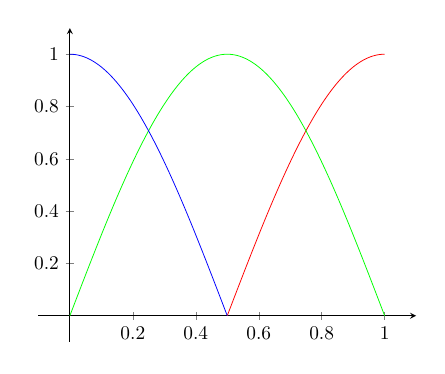
\begin{tikzpicture}[scale=0.7]
			\begin{axis}[
				trig format plots=rad,
				axis lines = middle,
				enlargelimits,
				clip=false
				]
				\addplot[domain=0.5:1,samples=200,red] {sin(pi*x - pi/2.0)};
				\addplot[domain=0:1,samples=200,green] {sin(x*pi)};
				\addplot[domain=0:0.5,samples=200,blue] {sin(pi*x + pi/2.0)};
				
			\end{axis}
		\end{tikzpicture}
	\caption{\textit{Mapping function from pixel difference to RGB components}}
	\label{fig:heat_sine}
	\end{figure}

	A second implementation, that is used to speed up the computation is to turn in red all pixels that are above a certain threshold. Obviously, the complexity of this computation is much easier than the previous one and in the CPU allows to compute that kind of map in around 300ms.
	\begin{figure}[H]
		\centering
		\includegraphics[width=0.4\linewidth]{images/heatmap/v0-red}
		\caption{\textit{All non normalized pixel difference are turned to red if above a certain threshold, in this case 30}}
		\label{fig:v0-red}
	\end{figure}

	The two implementations are manged via some compiler directives that allows to increase the performance, since only one of them can be visualized. The purpose of them is completely different, since the original heat map, the one explained at the beginning is used to understand the magnitude of the pixel difference while the second one (the black-red) is used to better visualize the noise pixels, by using a threshold. This allows to have a visual evaluation of the noise filter, that will be explained in the next section.
	
	\subsection{CUDA heat map implementation}
	The first implementation of the algorithm in CUDA is based on a 1:1 transposition of what done in the CPU, in the GPU. Always using OpenCV, two next frames are fetched, send to the kernel and the heat map computed.\newline\newline
	Unfortunately, the type problem doesn't need any shared memory because each location in the image (all three colors of all pixels) are accessed only one and using a shared memory would have only reduced the performance due to an useless copy.
	
	In order to speed up the data management, instead of copying into a support array of \texttt{uint8\_t} the entire two frames (previous and current), are directly copied into the device buffers with the \texttt{cudaMemcpy} procedure. The program is named \texttt{v1.cu} and can be compiled with the \texttt{make build-v1} command.
	
	After having run the \texttt{nvprof}, the main contribution to the execution time from the profiler are:
	\begin{figure}[H]
		\centering
			\begin{center}
			\begin{tabular}{ |c|c|c|c| } 
				\hline
				\textbf{Type} & \textbf{Time} (\%) & \textbf{Avg} & \textbf{Name} \\ 
				\hline
				GPU activities & 80.62 & 31.486ms & kernel \\ 
				& 13.20 & 2.578ms & [CUDA memcpy HtoD] \\ 
				& 6.18 & 2.4136ms & [CUDA memcpy DtoH] \\ 
				\hline
				API calls & 93.47 & 13.664ms & cudaMemcpy \\ 
				& 6.22 & 123.70ms & cudaMalloc \\ 
				\hline
			\end{tabular}
		\end{center}
		\label{fig:table_v1}
		\caption{\textit{Profiling result v1.cu}}
	\end{figure}
	In fact, the cumulative time needed to copy all two frames into the device, execute the kernel and copy back the image in order to display it, takes approximately 40ms.\newline\newline
	Instead of copying each time both the two frame, one of the two can be reused by only switching the two points, so that the one that previously was the current will became the previous; at this point, only the new frame must be copied into the device memory. This means that approximately the \textit{CUDA memcpy HtoD} should be half of the previous time. This led to a \texttt{v2.cu} implementation, that exploit this pointer switching to reduce the memory transfer.
	\begin{figure}[H]
		\centering
		\begin{center}
			\begin{tabular}{ |c|c|c|c| } 
				\hline
				\textbf{Type} & \textbf{Time} (\%) & \textbf{Avg} & \textbf{Name} \\ 
				\hline
				GPU activities & 87.69 & 31.786ms & kernel \\ 
				& 6.25 & 2.4276ms & [CUDA memcpy HtoD] \\ 
				& 6.18 & 2.3777ms & [CUDA memcpy DtoH] \\ 
				\hline
				API calls & 87.88 & 20.249ms & cudaMemcpy \\ 
				& 11.84 & 182.85ms & cudaMalloc \\ 
				\hline
			\end{tabular}
		\end{center}
		\label{fig:table_v2}
		\caption{\textit{Profiling result v2.cu}}
	\end{figure}
	The average times in ms, are not a figure of interest, since are more or less equal to the previous version. What is important is that now, the percentage of time used for the kernel is increase, due to the reduced \textit{CUDA memcpy HtoD} (from 13.20\% to 6.25\%). This means that the GPU will analyze more frame in the same time frame. As we would expect, now the time needed to copy a frame from the memory to the device, execute the kernel and then retrieve the heat map takes about 36ms (10\% faster).\newline\newline
	In order to reduce the number of accesses to memory, the idea was to access at the int level instead of the byte level. This means that frame information are still copied from host to device as arrays of bytes but they are accesses at the int level. So, if the current and the previous frames are passed as \texttt{uint8\_t *current, uint8\_t *previous}, the access is aligned at the 4 bytes in the following way:\newline\newline		\texttt{cc = ((int *)current)[i];}\newline
	\texttt{pc = ((int *)previous)[i];}\newline\newline
	This led to another version, available at \texttt{v3.cu} allows to obtain the following results:
	\begin{figure}[H]
		\centering
		\begin{center}
			\begin{tabular}{ |c|c|c|c| } 
				\hline
				\textbf{Type} & \textbf{Time} (\%) & \textbf{Avg} & \textbf{Name} \\ 
				\hline
				GPU activities & 81.28 & 21.071ms & kernel \\ 
				& 9.52 & 2.4599ms & [CUDA memcpy HtoD] \\ 
				& 9.19 & 2.383ms & [CUDA memcpy DtoH] \\ 
				\hline
				API calls & 93.63 & 13.644ms & cudaMemcpy \\ 
				& 5.89 & 171.89ms & cudaMalloc \\ 
				\hline
			\end{tabular}
		\end{center}
		\label{fig:table_v3}
		\caption{\textit{Profiling result v3.cu}}
	\end{figure}
	
	This version allows to copy the next frame from memory to device, execute the kernel and retrieve the result in about 26ms (about 28\% of performance increase from \texttt{v2.cu}). This is highlighted in the table by the average time needed to execute the kernel itself, we went from 31.786ms to 21.071ms.\newline\newline
	\textbf{TODO try streams + trye set number of threads to maximum}
	
\end{document}